\documentclass[]{beamer}
\usepackage[T1]{fontenc}
\usepackage[utf8]{inputenc}
\usepackage{lmodern}
\usepackage[italian]{babel}
\usepackage{mathrsfs}
\usepackage{cancel}

\title{Il potenziale elettrico}
\author{\texorpdfstring{Mattia Cozzi\newline\href{mailto:cozzimattia@gmail.com}{\texttt{cozzimattia@gmail.com}}}{Mattia Cozzi}}
\date{a.s.~2023/2024}

%\documentclass[handout]{beamer}     %usare questa classe per generare l'handout
%\usepackage{pgfpages}   %per mostrare più quadri nella stessa pagina
%\pgfpagesuselayout{4 on 1}[a4paper,border shrink=5mm,landscape]
\usetheme{Singapore}
%\useoutertheme[left]{sidebar} %elementi intorno alle diapositive
\setbeamercovered{dynamic} %modifica l'aspetto del testo grigetto delle diapositive future. Argomenti: invisible/transparent/dynamic
\usecolortheme{orchid}
% %COLORE PRINCIPALE
% \definecolor{marroncino}{RGB}{156, 26, 0} % UBC Blue (primary)
% \setbeamercolor{structure}{fg=marroncino} % itemize, enumerate, etc

\theoremstyle{plain}
\newtheorem{teorema}{Teorema}

\usepackage{tikz}
\usepackage{circuitikz}

\usepackage{pgf,pgfplots,graphicx}
\usetikzlibrary{angles,quotes,arrows,shapes,decorations.markings}
\pgfplotsset{compat=1.15}
\usepgfplotslibrary{units,fillbetween} % to add units easily to axis

\newcommand{\fem}{f_{em}}

\def\angolo[#1](#2)(#3:#4:#5)% Syntax: [draw options] (center) (initial angle:final angle:radius)
    { \draw[#1] ($(#2)+({#5*cos(#3)},{#5*sin(#3)})$) arc (#3:#4:#5); }


\begin{document}

\begin{frame}
  \titlepage
\end{frame}





\begin{frame}
\frametitle{Contenuti}
\tableofcontents
\end{frame}


\section{Energia potenziale}

\begin{frame}
\frametitle{Forze conservative}
Sappiamo che la forza di gravità è una forza conservativa:
\begin{block}{Definizione}
Una forza si dice conservativa se il \emph{lavoro} che essa fa nello spostamento del suo punto di applicazione da un punto $ A $ fino a un punto $ B $ dipende soltanto dalle posizioni $ A $ e $ B $, ma non dal particolare percorso seguito durante lo spostamento.
\end{block}\pause
Analogamente, anche la forza di Coulomb è conservativa, e possiamo definire per essa una \alert{energia potenziale}.
\end{frame}


\begin{frame}
\frametitle{Energia potenziale di due cariche (1)}
Immaginiamo un sistema di due cariche puntiformi, $ q_1 $ e $ q_2 $, poste a distanza $ r $.
\begin{figure}
\begin{tikzpicture}[scale=0.5]
\draw [] (6,0) -- (0,0);
\node [above,red] at (6,.3) {$ q_2 $};
\draw [red, ultra thick,fill=red] (6,0) circle [radius=.3];
\node [above] at (3,0) {$ r $};
\node [above,red] at (0,.3) {$ q_1 $};
\draw [red, ultra thick,fill=red] (0,0) circle [radius=.3];
\end{tikzpicture}
\end{figure}\pause
Definiamo l'energia potenziale elettrica del sistema come:
\begin{center}
\colorbox{blue!30}{$ U(r) = k_0 \dfrac{q_1 \, q_2}{r} $}
\end{center}
\end{frame}



\begin{frame}
\frametitle{Energia potenziale di due cariche (2)}
Nella definizione precedente, abbiamo assegnato il valore $ 0 $ dell'energia potenziale alla situazione in cui le due cariche sono a distanza infinita.
\pause

~

In effetti:
\begin{center}
$ \displaystyle \lim_{r \to + \infty} k_0 \dfrac{q_1 \, q_2}{r} = 0 $
\end{center}\pause

\begin{block}{Definizione di energia potenziale elettrica}
L'energia potenziale elettrica è il lavoro compiuto dalla forza di Coulomb quando le cariche sono portate a distanza infinita tra loro.
\end{block}
\end{frame}


\begin{frame}
\frametitle{Approfondimento (1)}
Se due cariche vengono allontanate, la forza elettrica agente su di esse cambia secondo la funzione:
\begin{center}
$ F(x) = k_0 \dfrac{q_1 \, q_2}{x^2} $
\end{center}\pause
Poiché tale forza è variabile, il lavoro tra il punto $ A $ e il punto $ R $ di riferimento (a distanza infinita) verrà calcolato come somma di tutti i lavori elementari tra $ A $ ed $ R $:
\begin{center}
$ U(A) = \displaystyle \int_A^R \vec{F}(x) \cdot d \vec{s}  $ 
\end{center}\pause
Poiché $ \vec{F} $ e $ \vec{s} $ sono paralleli, vale:
\begin{center}
$ U(A) = \displaystyle \int_A^R F(x) d x  $ 
\end{center}
\end{frame}



\begin{frame}
\frametitle{Approfondimento (2)}
Calcoliamo l'integrale definito:
\begin{center}
$ U(r) = \displaystyle \int_r^{r_0} F(x) dx = \int_r^{r_0} k_0 \dfrac{q_1 \, q_2}{x^2} dx =  $ \pause

~

~

$  = \left[ - k_0 \dfrac{q_1 \, q_2}{x} \right]^{r_0}_r =  - k_0 \dfrac{q_1 \, q_2}{r_0} + k_0 \dfrac{q_1 \, q_2}{r}  $
\end{center}\pause
Ponendo $ - k_0 \dfrac{q_1 \, q_2}{r_0} = 0 $ otteniamo
\begin{center}
$ U(r) = \displaystyle  k_0 \dfrac{q_1 \, q_2}{r} $ 
\end{center}
\end{frame}



\begin{frame}
\frametitle{Segno dell'energia potenziale}


\begin{columns}
\begin{column}{0.3\textwidth}
\begin{figure}
\begin{tikzpicture}[xscale=.7,yscale=.7]
\draw [->] (-.15,0) -- (3.5,0);
\draw [->] (0,-.15) -- (0,3.5);
\draw[smooth, red, thick, domain=0.1:3, samples=50] plot 
({\x},{ ((3*\x))^-1 });
\node [below] at (3.5,0) {{\tiny $ r $}};
\node [left] at (0,3.5) {{\tiny $ U(r) $}};
\end{tikzpicture}

~

\visible<2>{\begin{tikzpicture}[xscale=.7,yscale=.7]
\draw [->] (-.15,0) -- (3.5,0);
\draw [<-] (0,.35) -- (0,-3.5);
\draw[smooth, blue, thick, domain=0.1:3, samples=50] plot 
({\x},{ ((-3*\x))^-1 });
\node [below] at (3.5,0) {{\tiny $ r $}};
\node [left] at (0,-3.5) {{\tiny $ U(r) $}};
\end{tikzpicture}}
\end{figure}
\end{column}
\begin{column}{0.6\textwidth}
\begin{center}
$ U(r) = k_0 \dfrac{q_1 \, q_2}{r} $
\end{center}

~

~

Se le due cariche hanno lo stesso segno l'energia potenziale è positiva.\pause

~

~


\visible<2>{Se le due cariche hanno segno opposto l'energia potenziale è negativa.}

~

~

~
\end{column}
\end{columns}
\end{frame}




\begin{frame}
\frametitle{Energia potenziale di sistemi complessi}
In sistemi con tre o più cariche, l'energia potenziale del sistema sarà la somma delle energie potenziali calcolate per ogni possibile coppia di cariche.

\begin{figure}
\begin{tikzpicture}[scale=0.5]
\draw [] (6,0) -- (0,0);
\draw [] (6,0) -- (4,3);
\draw [] (4,3) -- (0,0);
\node [below,red] at (6,-.3) {$ q_2 $};
\draw [red, ultra thick,fill=red] (6,0) circle [radius=.3];
\node [below] at (3,0) {$ r $};
\node [above] at (2,1.6) {$ s $};
\node [above] at (5.1,1.5) {$ t $};
\node [below,red] at (0,-.4) {$ q_1 $};
\node [above,red] at (4,3.2) {$ q_3 $};
\draw [red, ultra thick,fill=red] (0,0) circle [radius=.4];
\draw [red, ultra thick,fill=red] (4,3) circle [radius=.2];
\end{tikzpicture}

~

$ U = \left( k_0 \dfrac{q_1 \, q_2}{r} \right) + \left( k_0 \dfrac{q_1 \, q_3}{s} \right) + \left( k_0 \dfrac{q_2 \, q_3}{t} \right) $

\end{figure}
\end{frame}



\section{Potenziale}

\begin{frame}
\frametitle{Sistema di cariche e carica di prova}
Immaginiamo un sistema formato da $ Q_1 $, $ Q_2 $ e $ Q_3 $, a cui viene avvicinata una carica di prova $ q_p $ posta nel punto $ A $.

\begin{figure}
\begin{tikzpicture}[scale=0.4]
\draw [] (8,-2) -- (-2,-2) -- (-2,5) -- (8,5) -- (8,-2);
\node [below] at (3,-2) {{\footnotesize sistema di cariche}};
\node [below,red] at (6,-.3) {$ Q_2 $};
\draw [red, ultra thick,fill=red] (6,0) circle [radius=.3];
\node [below,red] at (0,-.4) {$ Q_1 $};
\node [above,red] at (4,3.2) {$ Q_3 $};
\node [above,red] at (11,1.1) {$ q_p $};
\node [below] at (11,.9) {$ A $};
\draw [red, ultra thick,fill=red] (0,0) circle [radius=.4];
\draw [red, ultra thick,fill=red] (4,3) circle [radius=.2];
\draw [red, ultra thick,fill=red] (11,1) circle [radius=.1];
\end{tikzpicture}
\end{figure}\pause

Calcoliamo l'energia potenziale del sistema formato da $ Q_1 $, $ Q_2 $, $ Q_3 $ e $ q_p $ e indichiamola con $ U_A $.
\end{frame}


\begin{frame}
\frametitle{Potenziale elettrico}
Definiamo il potenziale elettrico $ V_A $ del punto $ A $ come:
\begin{center}
\colorbox{blue!30}{$ V_A = \dfrac{U_A}{q_p} $}
\end{center}
Il potenziale elettrico si misura in \emph{volt}: $ 1 \, V = 1 \, \dfrac{J}{C} $.\pause

~

Contrariamente a quanto possa sembrare dalla definizione, \alert<2>{il potenziale elettrico nel punto $ A $ non dipende dalla carica di prova}, ma solo dalla posizione del punto $ A $ rispetto al sistema di cariche.
\pause

~

Lo dimostriamo per un sistema semplice, formato da \alert<3>{una carica puntiforme $ Q $ e da una carica di prova $ q_p $}.
\end{frame}


\begin{frame}
\frametitle{Potenziale di una carica puntiforme}
Poniamo la carica di prova in un punto $ A $, definito dalla sua distanza $ r $ dalla carica sorgente $ Q $.
\begin{figure}
\begin{tikzpicture}[scale=0.5]
\draw [] (6,0) -- (0,0);
\node [above,red] at (6,.1) {$ q_p $};
\node [below] at (6,-.1) {$ A $};
\draw [red, ultra thick,fill=red] (6,0) circle [radius=.1];
\node [above] at (3,0) {$ r $};
\node [above,red] at (0,.3) {$ Q $};
\draw [red, ultra thick,fill=red] (0,0) circle [radius=.3];
\end{tikzpicture}
\end{figure}\pause
Calcoliamo il potenziale in $ A $:
\begin{center}
$ V(r) = \dfrac{U_A}{q_p} = \dfrac{k_0 \dfrac{Q \, \cancel{q_p} }{r}}{\cancel{q_p}} $ ~~~\pause$ \Longrightarrow  $~~~ \colorbox{blue!30}{$ V(r) = k_0 \dfrac{Q}{r} $} 
\end{center}
Notiamo che \alert<3>{tale valore non dipende da $ q_p $, ma solo dalla posizione di $ A $ rispetto a $ Q $ (cioè da $ r $)}.
\end{frame}





\begin{frame}
\frametitle{Esempio 1}

\begin{exampleblock}{Potenziale in un punto}
{\small Calcola il potenziale in un punto $ P $ posto a distanza $ r = 7,32 \, cm $ da una carica $ Q = - 58,4 \, nC $.}
\end{exampleblock}
\pause
Dalla formula precedente:
\begin{center}
$ V = k_0 \dfrac{Q}{r} = 8,99 \times 10^9 \, \frac{Nm^2}{C^2} \cdot \dfrac{-5,84 \times 10^{-8} \, C}{7,32 \times 10^{-2} \, m} = $\pause

~

$ = - 7,17 \times 10^3 \, \dfrac{N m^{\cancel{2}}}{C^{\cancel{2}}} \cdot \dfrac{\cancel{C}}{\cancel{m}} = -7,17 \times 10^3 \, \dfrac{J}{C} = -7,17 \times 10^3 \, V $
\end{center}
\end{frame}


\section{Tensione}

\begin{frame}
\frametitle{Differenza di potenziale (tensione)}

Se spostiamo la carica di prova dal punto $ A $ al punto $ B $ possiamo definire la \emph{differenza di potenziale tra $ A $ ed $ B $}:
\begin{center}
$ \Delta V_{AB} = V_B - V_A = \dfrac{U_B}{q_p} - \dfrac{U_A}{q_p} = \dfrac{\Delta U_{AB}}{q_p}$
\end{center}\pause

~

\alert{La differenza di energia potenziale} tra $ A $ e $ B $ al numeratore \alert{è il lavoro compiuto dalla forza elettrica} nello spostare la carica da $ B $ ad $ A $.
\begin{center}
\colorbox{blue!30}{$ \Delta V_{AB} = \dfrac{L_{B \to A}}{q_p} = -\dfrac{L_{A \to B}}{q_p} $}
\end{center}
\end{frame}


\begin{frame}
\frametitle{Moto spontaneo delle cariche (1)}
Avremo un moto spontaneo di cariche quando il lavoro della forza elettrica è positivo (come accade ad esempio per un oggetto ad una certa altezza che cade per effetto della forza di gravità).\pause

~

Poiché abbiamo due tipi di cariche, avremo due possibili moti spontanei:
\begin{itemize}
  \item \alert<2>{le cariche positive} si muoveranno spontaneamente da punti ad alto potenziale verso punti a basso potenziale (\alert<2>{``scendono'' lungo la differenza di potenziale});\pause
  \item \alert<3>{le cariche negative} si muoveranno spontaneamente da punti a basso potenziale verso punti ad alto potenziale (\alert<3>{``risalgono'' la differenza di potenziale});
\end{itemize}
\end{frame}



\begin{frame}
\frametitle{Moto spontaneo delle cariche (2)}
Se tra i punti $ A $ e $ B $ esiste una tensione $ \Delta V $ per cui \alert{$ V_A > V_B $} (cioè il punto $ A $ è ad alto potenziale e $ B $ è a basso potenziale), avremo i seguenti moti spontanei:
\begin{figure}
\begin{tikzpicture}[scale=0.5]
\draw [->,thick,gray] (3,0) -- (5,0);
\draw [->,thick,gray] (0,0) -- (-2,0);
\draw [|-|,thick] (-6,-2) -- (9,-2);
\node [below] at (1.5,-2.3) {$ \Delta V $};
\node [above,red] at (3,.2) {$ q_+ $};
\node [below] at (-6,0) {$ A $};
\node [below] at (9,0) {$ B $};
\draw [ultra thick,fill] (-6,0) circle [radius=.1];
\draw [ultra thick,fill] (9,0) circle [radius=.1];
\draw [red, ultra thick,fill=red] (3,0) circle [radius=.2];
\node [above,blue] at (0,.2) {$ q_- $};
\draw [blue, ultra thick,fill=blue] (0,0) circle [radius=.2];
\end{tikzpicture}
\end{figure}
\end{frame}





\begin{frame}
\frametitle{Esempio 2}

\begin{exampleblock}{Moto di un elettrone}
{\small Un elettrone  viene spostato da una differenza di potenziale $ \Delta V = 2,3 \times 10^5 \, V $ tra i punti $ A $ e $ B $.
\begin{itemize}
  \item Quanta energia cinetica acquista?
  \item Qual è la sua velocità finale?
\end{itemize}}
\end{exampleblock}
\pause
L'energia cinetica acquistata è il lavoro fatto dalla forza elettrica tra il punto $ B $ e il punto $ A $:
\begin{center}
$ \Delta V_{AB} = - \dfrac{L_{A \to B}}{q} $~~~ $ \Longrightarrow  $ ~~~$ \Delta K = -q \Delta V  $\pause

$ \Delta K = - (-1,60 \times 10^{-19} \, C) (2,3 \times 10 ^5 \, V) = 3,7 \times 10^{-14} \, J $
\end{center}\pause
Invertendo la formula per l'energia cinetica si trova la velocità.\hspace*{\fill}[$ 2,9 \times 10^{8} \, m/s $]
\end{frame}

\section{Superfici}

\begin{frame}
\frametitle{Superfici equipotenziali}
Analogamente a quanto fatto con le linee del campo elettrico, possiamo trovare un modo per visualizzare il potenziale elettrico.

\begin{block}{Superficie (linea) equipotenziale}
Una superficie (linea) equipotenziale è l'insieme dei punti dello spazio in cui il potenziale elettrico assume il medesimo valore.
\end{block}\pause
\begin{center}
$ V(r) = k_0 \dfrac{Q}{r} $
\end{center}
Possiamo dedurre che il potenziale assume lo stesso valore in tutti i punti alla stessa distanza $ r $ da $ Q $, definendo pertanto una \alert{superficie sferica}.
\end{frame}




\begin{frame}
\frametitle{Superfici equipotenziali e linee del campo}
\begin{columns}
\begin{column}{0.25\textwidth}
\begin{figure}
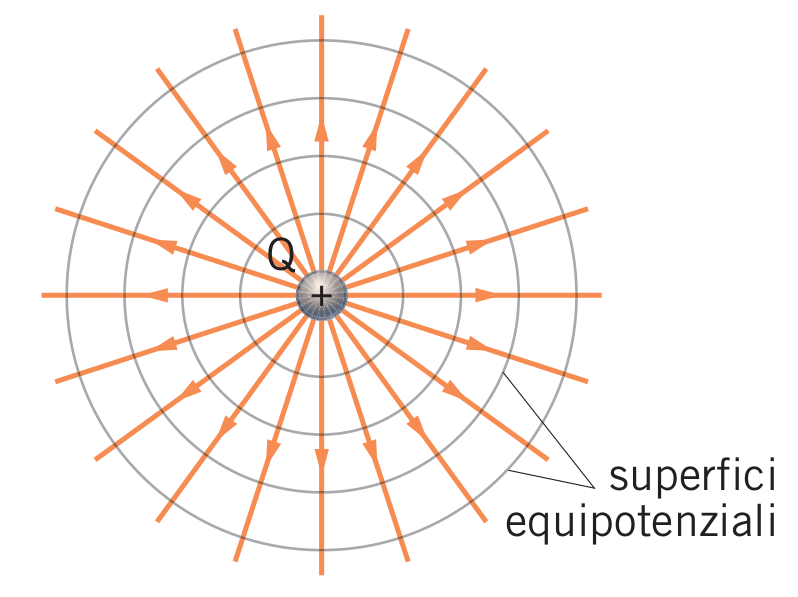
\includegraphics[width=\columnwidth]{img/superficieequipotenziale1.png}
\end{figure}
\end{column}
\begin{column}{0.25\textwidth}
\begin{figure}
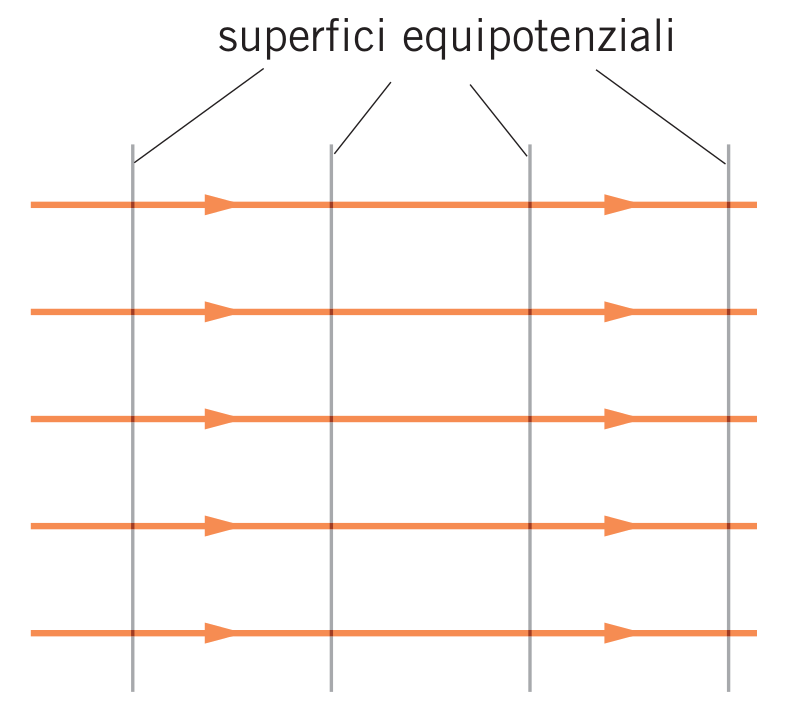
\includegraphics[width=\columnwidth]{img/superficieequipotenziale2.png}
\end{figure}
\end{column}
\begin{column}{0.5\textwidth}
\begin{figure}
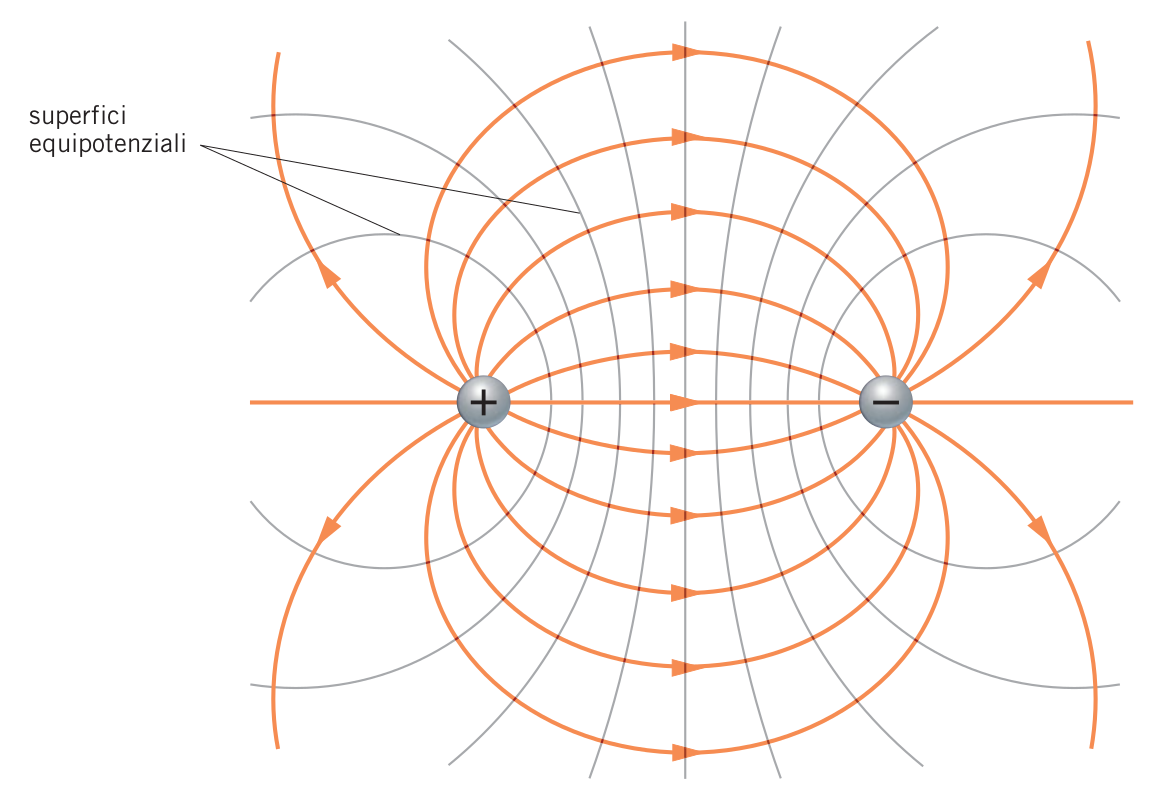
\includegraphics[width=\columnwidth]{img/superficieequipotenziale3.png}
\end{figure}
\end{column}
\end{columns}\pause

~

\alert{Le linee del campo elettrico sono sempre perpendicolari alle superfici (linee) equipotenziali.}\pause

~

Se infatti l'angolo tra $ \vec{E} $ e la superficie è di $ 90^\circ $, il lavoro della forza elettrica lungo la superficie sarà nullo e di conseguenza il potenziale rimarrà invariato.
\end{frame}







\section{Circuitazione}



\begin{frame}
\frametitle{Campo elettrico e potenziale elettrico}
Se una carica $ q $ si muove di un vettore $ \Delta \vec{s} $ in una zona dello spazio in cui il campo elettrico $ \vec{E} $ è uniforme, allora:
\begin{center}
$ L = \vec{F} \cdot \Delta \vec{s} = q\vec{E} \cdot \Delta \vec{s} $
\end{center}\pause
Poiché $ \Delta V = - \dfrac{L}{q} $, avremo:
\begin{center}
$ \Delta V = - \dfrac{\cancel{q}\vec{E} \cdot \Delta \vec{s}}{\cancel{q}} $ \pause$~~~~~ \Longrightarrow ~~~~~  $ \colorbox{blue!30}{$ \Delta V = - \vec{E} \cdot \Delta \vec{s} $} 
\end{center}\pause
Se lo spostamento avviene parallelamente al campo, la formula precedente si riduce a:
\begin{center}
\colorbox{blue!30}{$ \Delta V = - E \Delta s $} 
\end{center}
\end{frame}




\begin{frame}
\frametitle{Concetto di circuitazione}
\begin{figure}
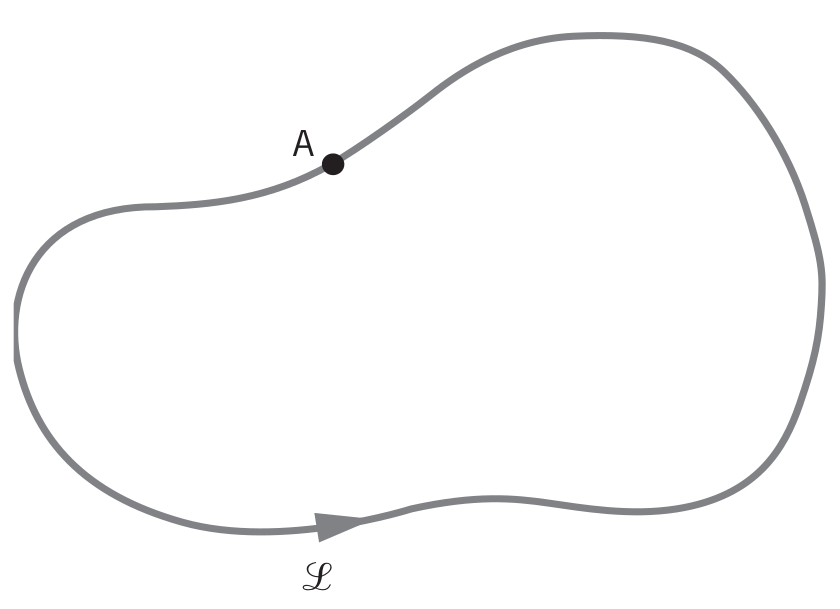
\includegraphics[width=.3\columnwidth]{img/lineachiusa.png}
\end{figure}
Quando abbiamo un campo elettrico $ \vec{E} $ che agisce in una certa zona dello spazio, risulta spesso utile valutare il suo andamento lungo una linea chiusa e orientata $ \mathscr{L} $.\pause

~

Introduciamo allora il concetto di \emph{circuitazione di un campo} lungo una linea $ \mathscr{L} $, con l'ipotesi che il campo sia costante nel tempo.
\end{frame}







\begin{frame}
  \frametitle{La circuitazione del campo elettrostatico (1)}
  Per calcolare la circuitazione del campo $ \vec{E} $ occorre scegliere arbitrariamente una linea chiusa e orientata $ \mathscr{L} $ e:\pause
  \begin{itemize}
    \item dividerla in $ n $ parti (al limite infinite) ognuna così piccola da poterla considerare \alert<2>{rettilinea} e \alert<2>{uniforme} il campo elettrico lungo di essa;\pause
    \item indicare con $ \Delta \vec{\ell}_i $ il \alert<3>{vettore spostamento} che descrive il tratto numero $ i $ di $ \mathscr{L} $;\pause
    \item determinare il vettore $ \vec{E}_i $, cioè il \alert<4>{campo elettrico lungo $ \Delta \vec{\ell}_i $};\pause
    \item calcolare il \alert<5>{prodotto scalare} $ \vec{E}_i \cdot \Delta \vec{\ell}_i $.
  \end{itemize}
\end{frame}


\begin{frame}
  \frametitle{La circuitazione del campo elettrostatico (2)}
  \begin{figure}
  \begin{tikzpicture}[xscale=.8,yscale=.8]
\draw [purple, thick] (0,0) circle [radius=3];
\angolo[black](7.5,1)(270:307:1)
\node [left, purple] at (-2.5,2) {$ \mathscr{L} $};
\draw (3,0) circle [radius=.2];
\draw (3,.2) -- (6.8,1.875);
\draw (3,-.2) -- (6.8,-1.875);
\draw (7.5,0) circle [radius=2];
\draw [thick, purple] (7.5,2)  -- (7.5,-2);
\draw [thick, blue, ->] (7.5,1)  -- (9,-1);
\node [left, purple] at (7.5,0) {{\scriptsize $ \Delta\vec{\ell}_i $}};
\node [right, blue] at (7.8,.8) {{\scriptsize $ \vec{E}_i $}};
\node [below] at (7.9,0.1) {{\scriptsize $ \theta_i $}};
\draw [thick, purple, ->] (-3,0)  -- (-3,.0001);
\end{tikzpicture}
\end{figure}
\begin{center}
   \colorbox{blue!30}{$ \Gamma_{\ell_i} (\vec{E}_i) = \vec{E}_i \cdot \Delta \vec{\ell}_i = E_i \ell_i \cos \theta_i $}
   \end{center}
\end{frame}




\begin{frame}
  \frametitle{La circuitazione lungo $ \mathscr{L} $}
  La circuitazione sarà la \alert<1>{somma di tutti i prodotti scalari}, calcolati per ogni tratto della linea $ \mathscr{L} $.
   \begin{center}
   \colorbox{blue!30}{$ \Gamma_\mathscr{L} (\vec{E}) = \sum\limits_{i=1}^n \vec{E}_i \cdot \Delta \vec{\ell}_i =  \sum\limits_{i=1}^n E_i \Delta \ell_i \cos\theta_i $}
   \end{center}
\end{frame}


\begin{frame}
  \frametitle{Il significato della circuitazione di $ \vec{E} $}
  Sappiamo che $ \vec{E}\cdot \Delta\vec{\ell} = - \Delta V $ e, indicando con $ \Delta V_i $  la differenza di potenziale tra gli estremi del segmento orientato $ \Delta \vec{\ell}_i $, avremo:
  \begin{center}
  $ \Gamma_\mathscr{L} (\vec{E}) = \sum\limits_{i=1}^n \vec{E}_i \cdot \Delta \vec{\ell}_i = \sum\limits_{i=1}^n (-\Delta V_i) = - \sum\limits_{i=1}^n \Delta V_i = 0 $
  \end{center}\pause
  La sommatoria delle differenze di potenziale lungo una linea chiusa è sempre nulla.\\\pause~\\
  
Ciò esprime matematicamente la proprietà del campo elettrostatico di essere \alert{conservativo}: il lavoro fatto dalla forza elettrica per spostare una carica non dipende dal percorso scelto ma solo dal punto di inizio e di fine (vale solo per il caso statico).
\end{frame}





\end{document}
